\chapter{Implementation} \label{chapter5}

This chapter will analyze ACS UPB Mobile from an architectural perspective, describing the framework based on its inner workings, data models, and design patterns. We will explain how we conceptualized and integrated the solution proposed in this paper to fully integrate with the codebase already existent and add further possibilities for improvement. 

\section{ACS UPB Mobile architecture} \label{4:app}

    \subsection{Database} \label{4:app:database}
 As every software solution needs a non-volatile storage environment, the application uses Firestore\footnote{https://firebase.google.com/docs/firestore/}, another component of the Google ecosystem. It is a modern cloud-based non-relational database designed to work with other Google SDKs, such as Flutter.
As a document-oriented database, its structure is based on two main components: documents and collections. Documents are files that contain the application data in a JSON-like format. 

Each document has a unique identifier and is composed of a list of pairs in the form of \textbf{keys} and \textbf{data}. A key is a unique string, and data can be of primitive and complex data types\footnote{https://firebase.google.com/docs/firestore/manage-data/data-types}, such as null, boolean, integer and double, date, string, and also Cloud Firestore reference, Array, and Map. A special feature is that documents don’t have a predefined format, so their structure can be easily manipulated.    
Collections are groups of documents that have a logical correlation with each other. As mentioned above, they don’t have to respect a strict structure, giving a significant level of liberty in implementation. 

~

One example that proves the advantage of using Flutter, which is also of interest for the purpose of this paper, is the database structure of university events.
As we will further elaborate on these \textbf{events}, for the moment, it suffices to know that, in the database, we use the \textbf{event} collection to save all the documents related to events. As we explained in an anterior chapter, in the application, we have different types of university events that require in the related document various fields. For instance, while an \textbf{All day event} requires just an end date, a \textbf{Recurring event} needs a recurrence rule\footnote{https://datatracker.ietf.org/doc/html/rfc5545\#section-3.3.10}. Instances of these events are saved into documents in the same collection and can be retrieved separately by doing queries that check the existence of a key-data pair in them.

While an old approach would be either creating different tables for these events or creating only one containing all the fields, it would raise many scalabilities and technical difficulties as data integrity checks and queries become complex. 
This solution is easily scalable, secure, and extensible \footnote{https://firebase.google.com/docs/firestore/security/rules-structure}, and in the next section, we will present how we integrated new events and collections.

    \subsection{Provider} \label{4:app:provider}
    As we remarked above, State management is vital to any Flutter application and can be done in different ways. The default way is using the InheritedWidget\footnote{https://api.flutter.dev/flutter/widgets/InheritedWidget-class.html}, a class that propagates changes down the components tree.
In ACS UPB Mobile, the State is managed with \textit{Provider}\footnote{https://pub.dev/packages/provider} and ChangeNotifer\footnote{https://api.flutter.dev/flutter/foundation/ChangeNotifier-class.html} classes, which are wrappers over InheritedWidget that significantly reduce the boiler-plate code and application complexity. 

A Provider’s core philosophy is being defined at the top of the branch that requires it, as it can be called from inner nodes. In the application, we define all the providers at the root of the application so that we can use them where they are needed. Appropriately named providers, they are composed of asynchronous methods that mainly interact with data transfers between the application and database. 

These asynchronous methods usually return a \textbf{Future} that behaves similarly to promises from Javascript\footnote{https://www.javascript.com/}. These Futures guarantee that the called method will finish, be it in an unknown time, and some data will be returned while the application continues to run. This type of behavior is vital, as it keeps the application running for the users while internally it waits for the transfer of data.

With providers defined at the top level, we want a way to update a branch of the application without refreshing the whole tree. This is where ChangeNotifer is used, as it restricts the refreshing behavior. Together with Provider, it assures that when a change is made, it notifies and propagates to all the branches that use it, so only they have to modify. 

Using this behavior, we can easily control the application tree’s State throughout the application tree while doing it in an optimal way.

\subsection{BLoC Design Pattern} \label{4:app:bloc}
 Knowing now that the providers are being used to transfer data between the user and the storage environment, we can present all the layers of the application. 
The application respects the BLoC design pattern presented earlier, as all the components use this three tyre approach.

~

\begin{wrapfigure}{r}{0.5\columnwidth}
            \centering
            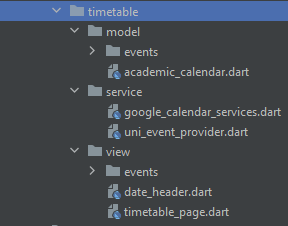
\includegraphics[width=0.5\columnwidth]{figures/c4/image5.png}
            \captionsetup{labelsep=space, textformat=empty}
            \caption{Screenshot of the events implementation}
            \label{4:bloc}
        \end{wrapfigure}
As we can see for example in figure \ref{4:bloc}, the timetable page is divided into three components :


\begin{itemize}
            \setlength{\topsep}{0.5pt}
            \setlength{\itemsep}{0.5pt}
            \setlength{\parsep}{0.5pt}
            \item Model, that is the equivalent of the data layer, where we can find the class definitions for the objects used inside the application. 
           \item Service, which can be considered the BLoC layer that handles the data transfers and communication between layers. 
            \item View, known as the presentation layer in this architecture, is where the code responsible for the interface can be found.
        \end{itemize}
        
\subsection{Flow} \label{4:app:flow}
We will now explain a general flow of the timetable component of the application concerning the design architecture. 
 	
 As we first access the timetable page, the View components start the initialization process. By having access to the provider, they ask the BLoC layer for data and receive a Future object, so the application doesn’t block while data is being retrieved. As the raw data is gathered from the database, it is then propagated to the data layer, where the object’s constructors can be found. When the object instances have been created, they are sent back to the BLoC layer to be delivered to the presentation layer. Finally, when the Future is solved, the view is complete, and the final data is presented to the user. 
	
This flow will also apply to features that we will implement for this paper’s purpose. 

\section{Integration strategy} \label{4:strategy}

In this section, we will describe the integration strategy of the proposed solution, as we want to follow the development principles and conventions that apply to ACS UPB Mobile. 
Going back to the proposed functionalities enumerated in the Introduction chapter, we will punctually explain how each had to be integrated.

The first proposed functionality was the integration of assignments as choosable event types for users. This implied the need for a new class for them, as we need additional data to translate a real-world university assignment into a digital representation correctly. Furthermore, these events have to be in the same collection as the other events and be retrieved and handled accordingly. We also need to address the creation, read, update, deletion as the new fields imply new data transfers checks.

The second proposed functionality deals with the overall planning of the events that the user wants to track. As a filter retrieves all the class events, a user might not want to see all of them, so we have to give them a more granular option that applies only to him. Creating a “hide” option for an event allows the user to choose what events he wants to see in his planner. Other widgets will be built for a more simplified way of actually seeing assignments and tasks.

The third proposed functionality deals with assisting the user in the solving process, as we want to give him more visibility over his work and advice over the implementation strategy. We want to create a new collection for these “goals”, where we can store data for each user, as this implementation leaves a possibility for new features like teams of students tracking one project and setting a common goal that each can follow. 

The fourth proposed functionality refers to statistics, and these can be generated based on the already available information. We need to decide what metrics are relevant and how to visually present them so the user can quickly understand the information. This process is only handled in the presentation layer, so no further integration is needed. 

~

The final goal is to integrate all that we proposed in the paper. This can be verified by using the GitHub platform to monitor the changes. In a following chapter, we will further expand the delivery process.


\section{Database integration} \label{4:database}

As we have access to the development database, we can directly interact with it, as we follow a basic guideline. Because our solution doesn’t change the flow of other components, we don’t want to modify already existing fields or structures, but to add new fields that help our new features.
We will enumerate the collections that have been changed or added and present their purpose.

~

\faDatabase \hspace{0.1cm} \textbf{\mintinline{text}{events}}

The events collection contains all of the academic events that the users have added. In the following table (\ref{4:tab:events}), we will present the structure of an task in the database. The elements changed or added in the development process of the solution described in this paper are highlighted with the color yellow.


\begin{table}[th]\small\linespread{1}
\caption{\textbf{Task} event structure}
\label{4:tab:events}
\begin{tabular}{| l | l | p{5.6cm} | p{2.6cm} |}
\hline
\textbf{Field} & \textbf{Type} & \textbf{Information } & \textbf{Example} \\
\hline
\hlslc{type} & \mintinline{text}{string} &  one of "homework", "project", "test" ,"administrative", "research" & “homework”
\\
\hline
addedBy & \mintinline{text}{string} & Id of the user that added it & "ti0QcVZFj
ZCtJ50WW6"
\\
\hline
calendar & \mintinline{text}{string} & The event must be correlated with an academic year & "2020"
\\
\hline
class & \mintinline{text}{string} & Name of the class & “L-A4-S2-PW-Tehnologia informaţiei”
\\
\hline
degree & \mintinline{text}{string} & Correlated learning cycle & “BSc” (bachelor's)
\\
\hline
relevance & \mintinline{text}{array<string>} & Filter relevance & [“C5”, “C1”]
\\
\hline
name & \mintinline{text}{string} & Name of the event & "Tema 1"
\\
\hline
duration  & \mintinline{text}{map<string, number>} & Explicit duration & \{“days”: 15, 
“months”: 2 \}
\\
\hline
\hlslc{location} & \mintinline{text}{string} & Link where the assignment can be found & “https://ocw.cs.
pub.ro/courses/
pw/tema1"
\\
\hline
\hlslc{editable} & \mintinline{text}{boolean} & If the event can be edited & true
\\
\hline
start & \mintinline{text}{timestamp} & Start date of the event. It must have a value & 14 May 2021 at 00:00:00 UTC+3
\\
\hline
\hlslc{softDeadline} & \mintinline{text}{timestamp} & Soft deadline of the event & 24 May 2021 at 00:00:00 UTC+3
\\
\hline
\hlslc{hardDealine} & \mintinline{text}{timestamp} & Hard deadline of the event & 28 May 2021 at 00:00:00 UTC+3
\\
\hline
\hlslc{grade}  & \mintinline{text}{number} & The maximum grade of the event & 4.5
\\
\hline 
\hlslc{penalties}  & \mintinline{text}{number} & Daily penalty points after the soft deadline & 0.1
\\
\hline
\end{tabular}
\end{table}
\clearpage

As we can see in table \ref{4:tab:events}, we had to add new event types, update the location field to accept links, and add new fields relevant only to tasks.
Deadlines represent precisely what they are named after, and we save penalties and grades inside the event. Finally, we use editable to add another layer of security over events, as maybe some of them should not be modified. 

~

\faDatabase \hspace{0.1cm} \textbf{\mintinline{text}{users}}

In the “users” collection, we find documents that contain user-specific information, such as classes and filters. However, as our new event types respect the general structure, they are already integrated with the filtering mechanism.

\begin{table}[th]\small\linespread{1}
\caption{\textbf{Users} new field}
\label{4:tab:users}
\begin{tabular}{| l | l | l | p{3.6cm} |}
\hline
\textbf{Field} & \textbf{Type} & \textbf{Information} & \textbf{Example} \\

\hline
permissionLevel & \mintinline{text}{number} & Permissions that the user has & 4
\\
\hline
... &&&
\\
\hline
\hlslc{hiddenEvents} & \mintinline{text}{array<string>} & List of id’s of hidden events & [“RN5jsfBHgDb”, “Reavx6YOEHSJJ” ]

\\
\hline
\end{tabular}
\end{table}

~
For the purpose of the new features, we only need to look at the new field added: \textbf{hiddenEvents} (table \ref{4:tab:users}), which is a list of the identifiers of the tasks that the users want to hide. 

~

\faDatabase \hspace{0.1cm} \textbf{\mintinline{text}{goals}}

A new collection that consists of documents that, for each user, remember what goals it has set for its events.

The structure of the document(table \ref{4:tab:goals}) :

\begin{table}[th]\small\linespread{1}
\caption{\textbf{Goals} structure}
\label{4:tab:goals}
\begin{tabular}{| l | l | p{5.6cm} | p{3.6cm} |}
\hline
\textbf{Field} & \textbf{Type} & \textbf{Information} & \textbf{Example} \\
\hline
addedBy & \mintinline{text}{string} & Id of owner has & "ti0QcVZFj
ZCtJ50WW6"
\\
\hline
taskGoals &\mintinline{text}{array<map>} & Each element of the array represent a goal for a task & table \ref{4:tab:goalstruct}
\\
\hline
\end{tabular}
\end{table}

~

\begin{table}[th]\small\linespread{1}
\caption{\textbf{taskGoals} structure}
\label{4:tab:goalstruct}
\begin{tabular}{| l | l | p{5.6cm} | p{3.6cm} |}
\hline
\textbf{Field} & \textbf{Type} & \textbf{Information} & \textbf{Example} \\
\hline
taskId & \mintinline{text}{string} & Id of related task & "RN5jsfBHgDb"
\\
\hline
targetGrade &\mintinline{text}{number} & The target grade & 4.5
\\
\hline
strategy &\mintinline{text}{string} & one of : "constant", "early", "late" & "constant" 
\\
\hline
\end{tabular}
\end{table}

~
By using this structure, we can independently store information about the user’s targets. Its main advantage is that we don’t expose more information necessary, leaving a place for collaborative tasks to be implemented.

The fields in table \ref{4:tab:goalstruct} are \textbf{targetGrade}, for establishing a goal to reach, and \textbf{strategy}, to establish how it can be reached. At the moment, we have three predefined strategies, giving advice on how reach the goal in with constant effort, or with more effort either earlier or later in regards to deadlines. 


\section{System integration} \label{4:system}

Concerning our solution, in this section, we will analyze the BLoC and Data layers implementation. 

We will break it down into two parts, methods that use already existing data and methods that use the new collections.

~

In the first part, we are interested in integrating a new type of event in the already existing pool of events. For this, we had to understand the mechanism of how the raw fetched data from the “events” collection is handled.

The general flow for events is :
\begin{itemize}
            \setlength{\topsep}{0.5pt}
            \setlength{\itemsep}{0.5pt}
            \setlength{\parsep}{0.5pt}
            \item The collection is retrieved from the database.
            \item We iterate through the documents and send them to the data layer so the corresponding events are created. In this step, we have to add a differentiator for tasks, and we do that by checking if the document retrieved has a \textbf{hardDeadline} field set, as it’s required and unique to only \textbf{tasks}.
            \item A stream of events is available to be consumed by other methods in the provider. 
\end{itemize}

As we mentioned previously, for every event type, there is a data model in the project. The one that was of interest to us is the \textbf{AllDayUniEvent}, as tasks are frequently spread throughout multiple days and end at midnight. 

Knowing this, we can consider the \textbf{AllDayUniEvent} as a parent class for our \textbf{TaskEvent}. Furthermore, AllDayUniEvent is a direct child of \textbf{UniEvent}, the general implementation of events inside the application. Therefore tasks are recognized as university events. One adaptation was required, as the \textbf{hardDeadline} for the task had to become the \textbf{endDate} in the \textbf{AllDayUniEvent} constructor, because both parameters are required. Besides this, the other specific data pairs described in the previous section were saved as instance fields.

Now that we have task events and other events, the next step is to create appropriate instances of these events. Every event has to have a generator of instances, as some events are recurring, and each instance has to exist independently. As tasks are not periodic, one task event generates one task event instance, creating an easily trackable one-to-one relationship between the two. 

Using this information, we created new methods in the events provider, most of which deal with selecting events from a date interval, events of a specific class, specific task. 

For example, as the mechanism works on Futures, once the events were selected, their instances were generated and then returned to the pages that need them. 
The same principles apply to the user provider when we update the hidden events list.

~

In the second part, we will analyze the process of creating the planner feature, ignoring the presentation layer for the moment, as it will be detailed in the next chapter. 

For the provider, we need to register it on the root of the application tree. We do that by using the \textbf{Multi Provider} functionality,  a list of multiple providers created at the start of the application, from the provider package. Having it registered, we can now use the provider inside the application.

The planner provider consists of methods that mainly deal with customization of tasks solving processes. It is only natural that we don’t alter the structure of events, so we have to create a new data model named \textit{Goal}. As presented above in database integration steps, a goal will follow the table \ref{4:tab:goals} structure.

We implemented the basic \textbf{CRUD}( create, read, update, delete) operations for goals inside the planner provider and conversions between data objects fetched from the database and instances to assure the integrity of the data transfer. Using these asynchronous methods, with others interacting with events visibility, we can solve complex processes with reduced effort.

~

We will describe the flow of operations from the BLoC and Data layers perspective, as the user wants to add a new goal for an event instance :  
\begin{itemize}
            \setlength{\topsep}{0.5pt}
            \setlength{\itemsep}{0.5pt}
            \setlength{\parsep}{0.5pt}
            \item The user opens the page of an instance of a task.
            \item The document that contains his goals is fetched from the database. A list of goals is created from the taskGoals field, and if that list includes a goal for the event that the user is interested in. 
            \item If the document doesn’t exist or the goal is not present in the list, a null value is returned, signaling that a goal is not set for the said event. 
            \item If the goal is not set yet, it adds a new goal for the task. The application checks the collection to find the user's document, and if not, creates one with an array of taskGoals of one element, the one that it had to be added. 
            \item If the document exists, the taskGoals list is fetched, the new event is added to it, and then saved in the database.
            \item If the event is already saved, now the user can simply update them.
\end{itemize}

With this flow, we can control the planner feature and help the user better schedule his assignments while effortlessly creating and updating them for all the users that follow the same classes. Diagrams for this process can be found in the appendix \ref{b:uml}.



